\chapter{はじめに}
本章では，本研究の研究背景，先行研究の課題，研究目的とリサーチクエスチョン，本研究の貢献，および論文構成について述べる．

\section{研究背景}
\subsection{メンタル不調の増加とストレス対処}
近年，精神的ストレスによるメンタル不調を抱える人は増加している．厚生労働省の資料によると，精神疾患を有する総患者数は平成14年の約258.4万人から増加を続け，平成29年には約419.3万人（入院30.2万人，外来389.1万人）に達している\cite{mhlw2022}．McEwen\cite{mcewen1998}は，ストレスが心身に及ぼす影響を「アロスタシス」と「アロスタティック負荷」の概念で説明した．アロスタシスとは，環境的・心理的・社会的な変化に適応するために身体が生理的な仕組みを動員して安定を保とうとする働きであり，それが過剰に働き続けた結果として身体に蓄積される負担がアロスタティック負荷である．慢性的なストレスは心血管疾患や免疫機能の低下，精神疾患のリスクを高めるため，日常の中で適切にストレスを和らげる手段をもつことは心身の健康を保つうえで重要である．

ストレスを和らげる手段としては，睡眠や運動に加えて，趣味や娯楽の活動が重視されている．趣味は，日常の役割から離れて自分のための時間をもつこと，好きなものに没頭すること，同じものを好きな人とつながることを通じて，気分の回復や生活の張りをもたらす．一方で，趣味は「やめれば済む」ものではなく，本人にとっての生きがいと結びついているため，その付き合い方は本人が自ら選ぶものである点に特徴がある．

\subsection{推し活の広がり}
現在の日本では，特定のアイドル，アニメ・漫画・ゲームのキャラクター，VTuberや配信者，俳優，声優，スポーツ選手などを継続的に応援する「推し活」が広く行われている．推し活には，楽曲や動画の視聴，ライブやイベントへの現地参加，CD・Blu-rayやグッズの購入，テレビ・ラジオ・雑誌のチェック，SNSでの情報収集と発信，ロケ地を訪れる「聖地巡礼」，ファンクラブへの入会，コラボカフェへの来店，二次創作など，多様な形態がある．

株式会社ロイヤリティ マーケティングが2023年に10〜60代の推し活経験者879名に行った調査では，約半数（50.7\%）が推し活によって生活費に影響を感じていると回答し，20〜40代では約4割が月5,000円以上を推し活に使っていた\cite{loyalty2023}．Z世代を対象とした調査でも，6割以上が「推し」をもった経験があり，推し活の意義として「毎日を楽しくするもの」が最も多く挙げられている\cite{mery2023}．市場の面でも，矢野経済研究所の調査によれば，2024年度の「アイドル」市場は前年度比23.7\%増と大きく伸びており，ファンとの関係を軸にした体験型の消費が広がっている\cite{yano2026}．ファンの消費行動は，単なる購買ではなく自己のアイデンティティを映す「鏡」としての意味をもつことも指摘されている\cite{sandvoss2005}．

\subsection{推し活の便益と負担}
推し活は，ファンに多くの便益をもたらす．推しの存在が毎日の活力となり，つらいときに気持ちを支え，同じ推しを応援する仲間とのつながりを生む．井上・上田\cite{inoue2023}は，アイドルに対するファンの心理的所有感（「自分たちの推し」という感覚）が幸福感と関連することを示し，上田・井上\cite{ueda2023}は，推し活意識が推しへの心理的所有感を介して幸福感を高めることを報告している．宮田\cite{miyata2024}も，推し活が幸福度にもたらす意味を考察している．女子大学生を対象とした市村\cite{ichimura2025}の調査は，推し活が「ファン活動」「オタク活動」とは異なる肯定的なイメージで捉えられていることを示した．

一方で，推し活は負担も生む．夜遅くまで配信を見たりSNSを追ったりすることによる睡眠不足，予算を超えたグッズの購入やくじへの出費，「すべてのイベントに参加しなければならない」「情報を追い続けなければならない」という義務感，SNS上で他のファン（同担）の活動を見て嫉妬したり落ち込んだりすること，ファン同士の人間関係の疲れなどである．本研究では，これらをまとめて「推し疲れ」と呼ぶ．推し疲れは，対人援助職などで研究されてきたバーンアウト（燃え尽き）\cite{maslach1981,kubo2007}と同様に，熱心に関わるほど生じやすいという特徴をもつと考えられる．

重要なのは，推し活では便益をもたらす活動と負担をもたらす活動が同じであることが多い点である．スクリーンタイムを制限するアプリや家計簿アプリは「減らすほど良い」ことを前提としているが，推し活において一律に活動を減らす助言をすると，負担だけでなく楽しさや生きがいまで失わせてしまう可能性がある．また，本人は自分のどの習慣が推し疲れにつながっているのかに気づきにくい．推し活を続けたまま負担を減らすには，その人の状態に合わせて「何をどう変えるか」を本人が選べる形で示す支援が必要である．

\subsection{筆者の前研究}
筆者は卒業研究\cite{imai2025thesis,imai2025hr}において，推し活時の心拍とストレスの関連を調べた．質問紙の回答から推し活のタイプを13種類に分類し，タイプの異なる体験者3名にスマートウォッチ（Garmin Vivosmart 4）を2週間装着してもらい，推し活前と推し活中の心拍数を比較した．その結果，1名では推し活前と推し活中の平均心拍数に有意差が認められたが，他の2名では認められなかった．また，主な推し活が動画視聴であったことから，受動的な推し活が副交感神経を優位にしてリラックスをもたらす可能性が考えられた一方，高ストレス状況下では推し活の肯定的な効果が抑えられる傾向も自由記述からうかがえた．

この前研究には，(1)体験者が3名と少なく統計的な一般化が難しいこと，(2)対象がライブやイベントのような能動的な推し活を含まない受動的な推し活に偏っていたこと，(3)期間が2週間と短く，継続的な効果を検証できなかったこと，(4)推し活の状態を測ることにとどまり，本人の推し活をより良くするための支援にはつながっていないこと，という課題が残った．本研究はこれらの課題を受け，多数のファンを対象とした調査と，個人に合わせた提案を行うシステムの構築・検証へと発展させるものである．

\section{先行研究の課題}
推し活やファン行動に関する先行研究（第2章で詳述）は，主に次の3点で課題を残している．

\begin{enumerate}
\item \textbf{便益と負担を同時に扱った定量的な検討が少ない．}多くの研究は推し活の動機や心理的な便益を扱うか，負担を個別に扱うにとどまり，同じ人の中で便益と負担がどのような行動から生じるのかを同時に分析した研究は少ない．
\item \textbf{個人差の扱いが記述にとどまる．}性格特性や心理的傾向とファン行動の関連は報告されているが，それを個人に合わせた支援にどう生かすか（性格を固定的な「タイプ」として扱うのか，行動と組み合わせて扱うのか）は実証的に検討されていない．
\item \textbf{個人を支援する仕組みがない．}パーソナルインフォマティクスの分野では，記録を見せるだけでは行動が変わりにくいことが知られている\cite{li2010,choe2014}．推し活においても，本人が自分の状態に気づき，自ら選んだ変更を試せるような支援の仕組みは検討されていない．
\end{enumerate}

\section{研究目的とリサーチクエスチョン}
本研究の目的は，多くのファンの性格特性・推し活行動・幸福度・推し疲れの関係を分析し，その知見に基づいて，本人が自ら選べる提案と「今のまま続けた場合」と「提案を取り入れた場合」の見込みを示すシステムOshiFitを構築し，その有用性を検証することである．OshiFitは，本人に似たアバターを用いて，プランA「現在のままの推し活」とプランB「最適化された推し活」の6週間後の幸福度と推し疲れの見込み（本研究ではこの差を「ウェルビーイング・ギャップ」と呼ぶ）を示す．これにより，本人が気づきにくい負担の原因に気づき，自ら選んだ小さな変更によって幸福度の向上とストレスの軽減につなげることをねらう．図\ref{fig:flow}に，OshiFitの5つの段階と本研究の各部分の対応を示す．

\begin{figure}[t]
\centering
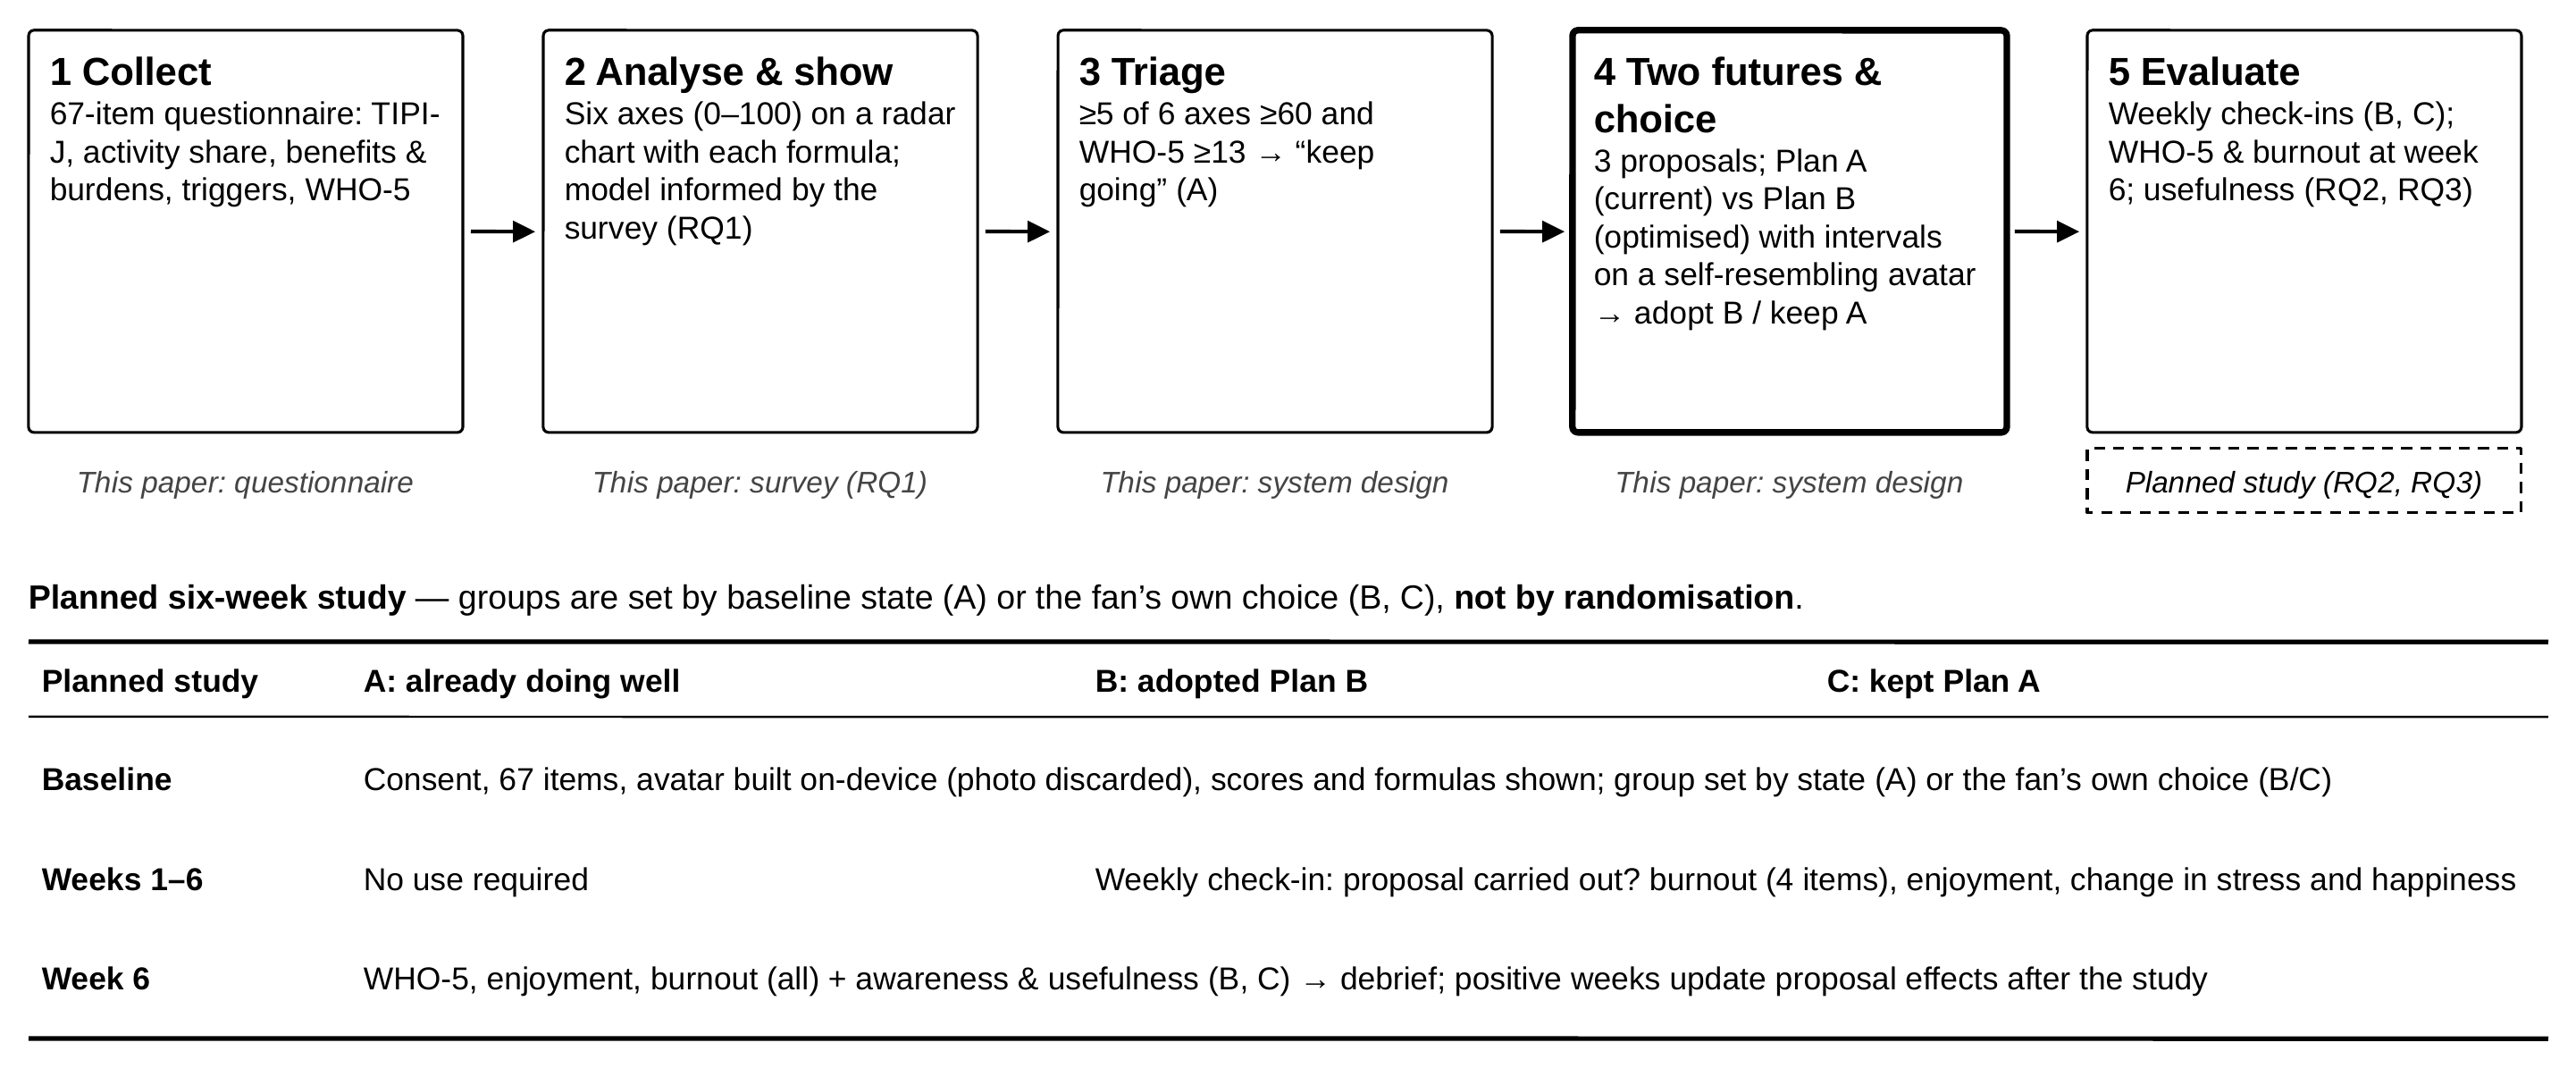
\includegraphics[width=\linewidth]{figures/fig1_flow_ppt.png}
\jecaption{OshiFitの5つの段階（上）と6週間の検証実験の計画（下）}{Five stages of OshiFit (top) and the planned six-week study (bottom)}
\label{fig:flow}
\end{figure}

本研究では，次の3つのリサーチクエスチョンを設定する．

\begin{description}
\item[RQ1] 性格特性（TIPI-J）と推し活行動は，幸福度・推し疲れとどのように関連し，個人の見込みとしてどの程度の精度で予測できるか．
\item[RQ2] 6週間の利用で，すでに良好な人（群A），プランBを選んだ人（群B），プランAを選んだ人（群C）の幸福度と推し疲れは，それぞれの群の中でどう変化し，群の間でどう異なるか．
\item[RQ3] 利用者は自分の推し疲れの原因に気づき，特に行動を変えた人はシステムを有用と評価するか．
\end{description}

RQ1には215名の質問紙調査で答え（第3章），その結果からシステムの設計指針を導いてOshiFitを構築する（第4章）．RQ2とRQ3には6週間の検証実験で答える（第5章）．

\section{本研究の貢献}
本研究の貢献は次の4点である．
\begin{enumerate}
\item 215名の調査により，推し活の便益（幸福度）と負担（推し疲れ）が同じ行動から生じることを定量的に示し，推し活の支援は「減らす」ことではなく「整える」ことを目指すべきであるという根拠を示した．
\item 性格特性は推し活の関わり方と関連するが，行動の効果を調整するわけではないことを示し，性格を固定的なタイプとしてではなく行動と組み合わせて個人化に用いるという設計の根拠を示した．
\item 個人の予測には大きな不確かさが伴うことを示し，予測を幅とともに正直に示す設計を導いた．
\item これらの知見を4つの設計指針にまとめ，本人に似たアバターで2つの未来を比較し，自ら選んだ行動変容を支援するシステムOshiFitを構築し，6週間の検証実験でその有用性を検討した．
\end{enumerate}

\section{論文構成}
本論文は全7章で構成される．第2章では，推し活・ファン行動，ウェルビーイングと負担，性格特性と個人化，パーソナルインフォマティクスと行動変容，アバターと将来の自己，予測の不確かさの提示に関する関連研究を概観し，本研究の位置付けを述べる．第3章では，RQ1に答えるための質問紙調査の方法と結果を述べ，システムの設計指針を導く．第4章では，OshiFitの設計と実装について述べる．第5章では，RQ2とRQ3に答えるための6週間の検証実験の方法と結果を述べる．第6章では，得られた知見を総合的に考察し，本研究の限界を述べる．第7章では，本研究をまとめ，今後の展望を述べる．
